\section{Rectificatifs du rapport de spécifications fonctionnelles}
\label{sec:rect}

\subsection{Architecture générale}
\label{subsec:archi}
La {\sc Figure} \ref{fig:archiPrevue} illustre l'architecture générale imaginée lors du rapport de spécifications fonctionnelles. Suite à des contraintes techniques, notamment dues au fait qu'un programme Java est difficilement contrôlable depuis un programme C\#, l'architecture a été revue pour correspondre à celle présentée à la {\sc Figure} \ref{fig:archiReelle}. ADTool ne fait finalement pas partie intégrante de Glasir, mais est lancé en tant que simple \og viewer \fg{} d'ADTree. En effet, il est impossible, depuis Glasir, de détecter des modifications faites dans ADTool, comme par exemple la modification d'une valuation de l'une des feuilles de l'ADTree. Par conséquent, la décision fut prise de désactiver toutes les fonctions d'édition dans ADTool lorsque Glasir se lance, donnant ainsi à ADTool un mode spécial batpisé \og viewmode \fg{} dans lequel l'utilisateur ne peut que visualiser un ADTree, sans pouvoir le modifier. De plus, la bibliothèque de modèles n'est également plus incluse dans Glasir, mais est simplement constituée d'un dossier contenant les fichiers des modèles, facilement importables. Ce dossier est fournit avec l'executable de Glasir.

		\begin{figure}[H]
            \centering
                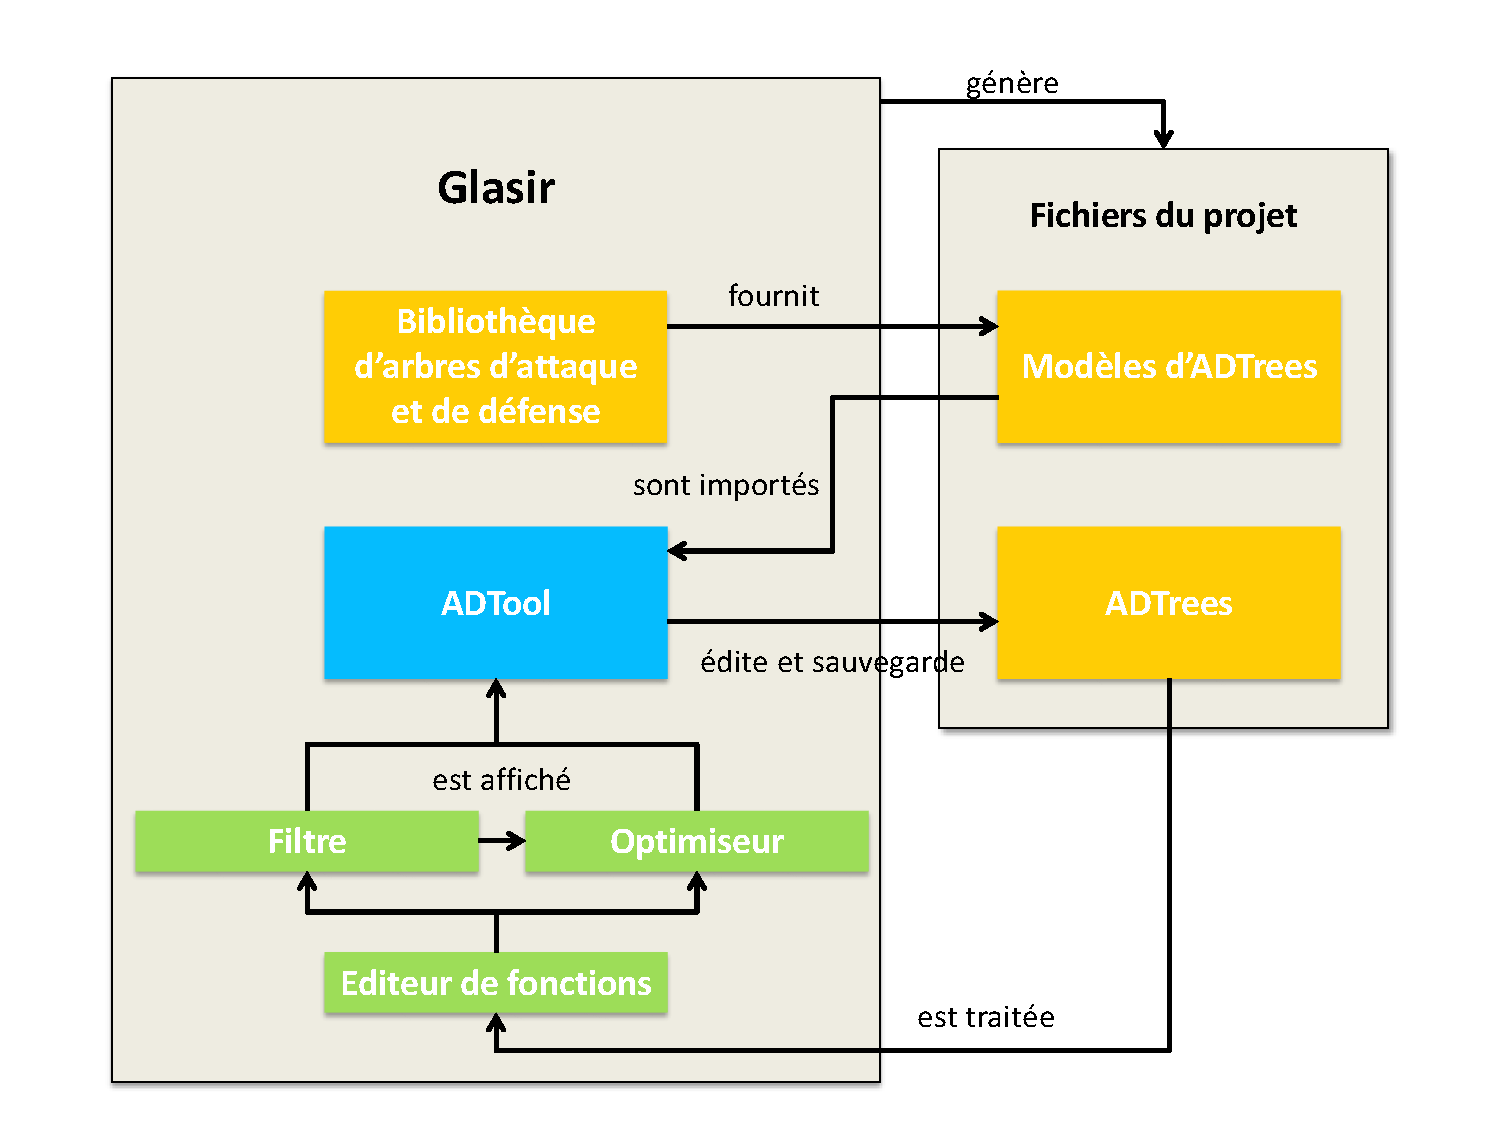
\includegraphics[width=0.8\textwidth]{figure/archiGlasir.pdf}
            \caption{Architecture initialement prévue.}
            \label{fig:archiPrevue}
        \end{figure}
	
        
        \begin{figure}[H]
            \centering
                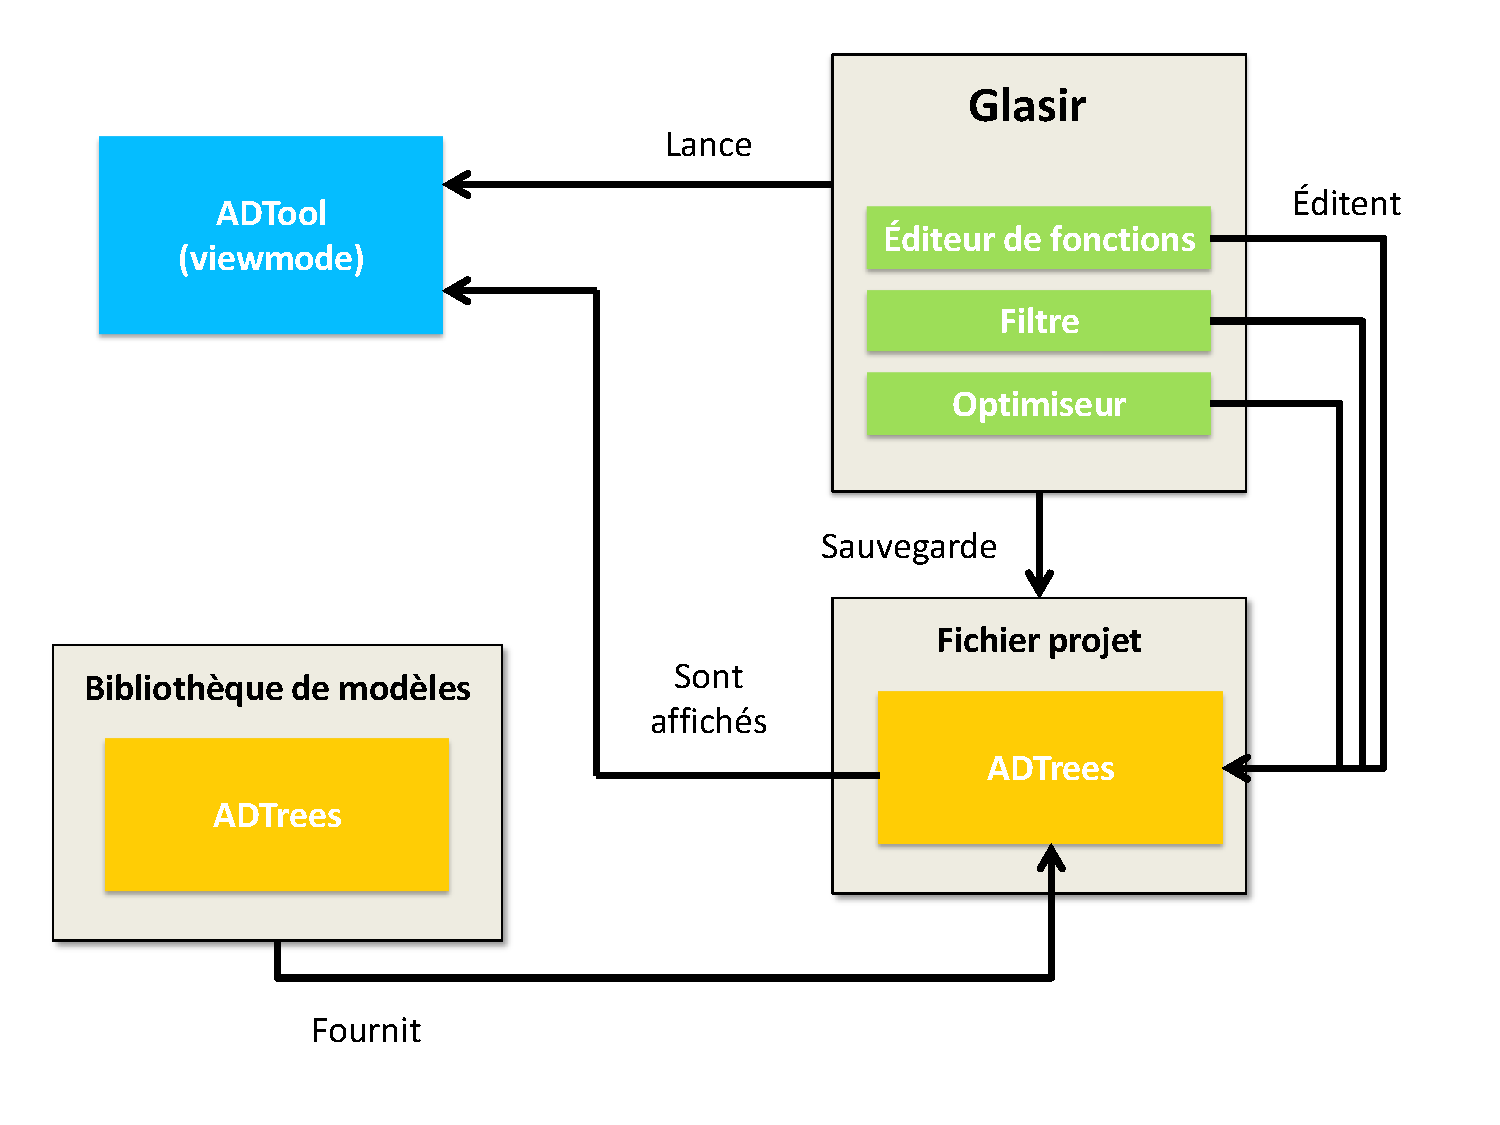
\includegraphics[width=0.8\textwidth]{figure/archiReelle.pdf}
            \caption{Architecture réelle.}
            \label{fig:archiReelle}
        \end{figure}
        
        
\subsection{Algorithme de l'Éditeur de fonctions}

Bien que nous n'ayons pas jugé interessant de détailler l'algortihme de l'éditeur de fonctions lors de la rédaction du rapport de spécification, celui ci s'est révélé plus délicat à implémenter que prévu et nous en détaillons donc le fonctionnement ici.

Algorithme implémenté pour l'éditeur de fonctions :

	\begin{algorithm}[h!]
            \caption{functionEdition(racine, param1, param2, function)}
            \label{algo:functionEdition}
            \begin{algorithmic}
		\IF{type(racine) == defense}
			\FORALL{sub IN fils(racine)}
				\STATE functionEdition(sub, param1, param2, function)
			\ENDFOR
			\RETURN
		\ENDIF
		\STATE
		\IF{type(racine) == feuille}
			\STATE p1 = param1(racine)
			\STATE p2 = param2(racine)
			\STATE newParam(racine) = function(p1,p2)
			\RETURN
		\ELSE
			\FORALL{sub IN fils(racine)}
				\IF {(type(sub) == defense}
					\STATE p1 = param1(racine)
					\STATE p2 = param2(racine)
					\STATE newParam(racine) = function(p1,p2)
				\ENDIF
				\STATE functionEdition(sub, param1, param2, function)
			\ENDFOR
		\ENDIF
            \end{algorithmic}
        \end{algorithm}

 Les notations non explicites sont présentées ci-dessous :
        \begin{itemize}
            \item \verb|racine| correspond au nœud racine de l'arbre ou sous-arbre manipulé ;
            \item \verb|param1| est une fonction renvoyant la valeur du premier paramètre qui nous intéresse pour un nœud donné ;
            \item \verb|param2| est une fonction renvoyant la valeur du second paramètre qui nous intéresse pour un nœud donné ;
            \item \verb|function| est une fonction prenant deux paramètres et calculant un résultat ;
            \item \verb|fils| est une fonction renvoyant la liste des fils du nœud passé en paramètre ;
            \item \verb|mode| précise si il s'agit d'un nœud disjonctif ou conjonctif ;
            \item \verb|type| précise si il s'agit d'un nœud d'attaque ou de défense, ou bien d'une feuille.
        \end{itemize}

\subsection{Algorithme du Filtre}

L'algorithme original du filtre comportait quelques erreurs, dont le fait pouvoir conserver des sous-noeuds d'un noeud conjonctif qui ne repectaient pas la condition de filtrage. Il a donc été modifié en conséquence.

Algorithme d'origine du filtre :

 	\begin{algorithm}[h!]
            \caption{filtre(racine, rules)}
            \label{algo:filtre}
            \begin{algorithmic}
                \FOR{r in rules}
                    \IF{not r(racine)}
                        \STATE delete(r) // will delete subtrees as well
                        \RETURN
                    \ENDIF
                \ENDFOR
                \STATE
                \FOR{n in fils(racine)}
                    \STATE filtre(n, rules)
                \ENDFOR
            \end{algorithmic}
        \end{algorithm}

Algorithme réellement implémenté :

 	\begin{algorithm}[h!]
            \caption{filtre(racine, param, max)}
            \label{algo:filtrereal}
            \begin{algorithmic}
	\STATE val = param(racine)
	\STATE
	\IF {val > max}
		\STATE delete(racine) // will delete subtrees as well
		\RETURN
	\STATE
	\ELSE
		\IF{mode(racine) == et}
			\FORALL{sub IN fils(racine)}
				\STATE subval = sub.param
				\STATE filtre(sub, param, max+subval-val)
			\ENDFOR
		\ELSE
			\FORALL{sub IN fils(racine)}
				\STATE filtre(sub, param, max)
			\ENDFOR
		\ENDIF
	\ENDIF
            \end{algorithmic}
        \end{algorithm}

        \begin{itemize}
            \item \verb|max| est la pire valeur pour le paramètre param que l'on désire dans l'arbre filtré peu importe le chemin envisagé.
        \end{itemize}

\subsection{Algorithme de l'Optimiseur}

Algorithme d'origine de l'optimiseur :

         \begin{algorithm}[h!]
            \caption{opti(racine, param)}
            \label{algo:opti}
            \begin{algorithmic}
                \STATE l\_fils = fils(racine)
                \IF{vide(l\_fils)}
                    \RETURN
                \ENDIF
                \STATE
                \IF{mode(racine) == ou}
                    \STATE v = param(racine)

                    \FOR{n in l\_fils}
                        \IF{not defense(n) and param(n) != v}
                            \STATE delete(n) // will delete subtrees as well
                        \ENDIF
                    \ENDFOR
                \ENDIF
                \STATE
                \FOR{n in fils(racine)}
                    \STATE opti(n, param)
                \ENDFOR
            \end{algorithmic}
        \end{algorithm}

Après reflexion, il nous est apparu que l'optimiseur tel que présenté dans le rapport de spécifiction pouvait être implémenté de manière bien plus simple, en se servant du filtre sans en impacter le résultat. Nous présentons donc ici le fonctionnement réel de l'optimiseur implémenté.

Algorithme réellement implémenté :

	\begin{algorithm}[h!]
            \caption{opti(racine, param)}
            \label{algo:optireal}
            \begin{algorithmic}
		\STATE v = param(racine)
		\STATE filtre(racine, param, v)
            \end{algorithmic}
        \end{algorithm}

\newpage
\section{Rectificatifs du rapport de conception}
\label{sec:rectConc}


	\subsection{Affichage multiple des paramètres}

	\subsection{Couper-copier-coller}
	La {\sc Figure} \ref{fig:copypastePrevu} illustre l'implémentation du couper-copier-coller imaginée lors du rapport de conception. Après s'être confronté à la réelle structure interne d'ADTool, il nous parut beaucoup plus simple de réaliser cette fonctionnalité comme indiqué sur la {\sc Figure} \ref{fig:copypasteReel}. Un ADTree est en réalité un \emph{ADTreeNode} possédant des fils, qui sont eux-même des \emph{ADTreeNode}. Cet ADTree est affiché à l'écran via un \emph{ADTreeCanvas}. Les actions au clavier et à la souris réalisées par l'utilisateur sont captées par la classe \emph{AbstractCanvasHandler}, qui possède le \emph{ADTreeCanvas} sur lequel agit l'utilisateur. Nous avons donc ajouté à l'\emph{AbstractCanvasHandler} un attribut de \emph{ADTreeTransferHandler}, une nouvelle classe qui contient les méthodes de copie et de collage d'un \emph{ADTreeNode}. Ainsi, lorsque l'utilisateur lance la commande couper, par exemple, la commande est captée par la classe \emph{CanvasHandler}, qui demande à sa classe parente (\emph{AbstractCanvasHandler}) de récuperer l'\emph{ADTreeNode} à couper (il s'agit de l'attribut \emph{focusedNode} de \emph{ADTreeCanvas}). L'\emph{ADTreeTransferHandler} se charge de l'opération de copie en stockant un clone de l'\emph{ADTreeNode} coupé, tandis que la suppression de l'ADTree coupé est gérée en interne par l'\emph{AbstractCanvasHandler}. Pour le collage, les opérations sont sensiblement identiques, sauf que le clone stocké par l'\emph{ADTreeTransferHandler} est restitué à l'\emph{AbstractCanvasHandler} qui se charge de l'ajouter à son \emph{ADTreeCanvas}.
	
	
		\begin{figure}
            \centering
                
\includegraphics[width=0.8\textwidth]{figure/copiercoller.png}
            \caption{Diagramme de classe prévu pour le couper-copier-coller.}
            \label{fig:copypastePrevu}
        \end{figure}
        
        \begin{figure}
            \centering
                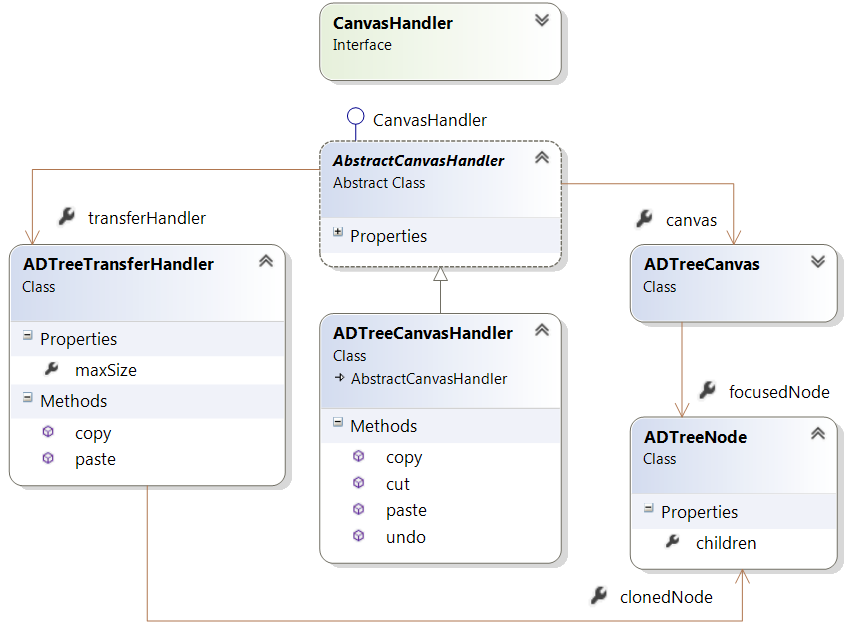
\includegraphics[width=0.8\textwidth]{figure/copiercollerReel.png}
            \caption{Diagramme de classe réel pour le couper-copier-coller.}
            \label{fig:copypasteReel}
        \end{figure}
       
	\subsection{Annulation des dernières actions}
		 La {\sc Figure} \ref{fig:ctrlzPrevu} illustre l'implémentation de l'annulation des dernières actions telle qu'imaginée lors du rapport de conception. De la même façon que pour le couper-copier-coller, la structure d'ADTool nous a poussé à implémenter l'annulation différemment, comme indiqué sur la {\sc Figure} \ref{fig:ctrlzReel}. En effet, associer chaque action à une classe se révélait trop fastidieux, étant donné le grand nombre d'actions possibles. L'\emph{AbstractCanvasHandler} se voit donc doté d'un attribut de \emph{UndoExecutor}, une nouvelle classe qui contient les méthodes d'annulation. Lorsque l'utilisateur réalise une action, un clone de l'ADTree est empilé dans la pile de l'\emph{UndoExecutor}. Les clones sont dépilés et rechargés dans l'\emph{ADTreeCanvas} lorsque l'utilisateur utilise la fonctionnalité d'annulation. Afin d'éviter une saturation de la mémoire, la pile ne peut contenir qu'un certain nombre de clones de l'ADTree, supprimant le plus ancien pour pouvoir empiler le plus récent. Il est à noter que plus l'ADTree est petit, plus le nombre d'actions annulables est grand, car la pile peut contenir plus de clones avant d'indiquer sa saturation. Dans le pire des cas, si l'ADTree est immense, seule la dernière action sera annulable. 
		 
        \begin{figure}
            \centering
                
\includegraphics[width=0.8\textwidth]{figure/ctrlz.png}
            \caption{Diagramme de classes prévu pour l'annulation des dernières actions.}
            \label{fig:ctrlzPrevu}
        \end{figure}
        
        \begin{figure}
            \centering
                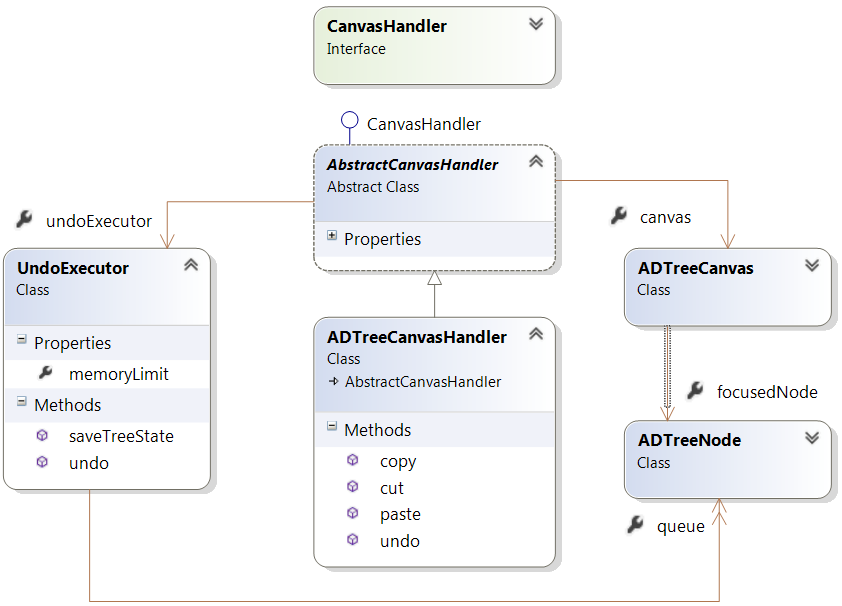
\includegraphics[width=0.8\textwidth]{figure/ctrlzReel.png}
            \caption{Diagramme de classes réel pour l'annulation des dernières actions.}
            \label{fig:ctrlzReel}
        \end{figure}

	\subsection{Bibliothèque de modèles}
		La {\sc Figure} \ref{fig:library} illustre l'implémentation de la bibliothèque de modèles telle qu'imaginée lors du rapport de conception. Finalement, cette bibliothèque se présente comme un simple dossier contenant les modèles, fourni avec Glasir. En effet, les contraintes décrites dans la {\sc section} \ref{subsec:archi} ayant imposé la création du \emph{viewmode} d'ADTool ont également nécessité de donner un tel format à la bibliothèque.
		
		\begin{figure}
            \centering
                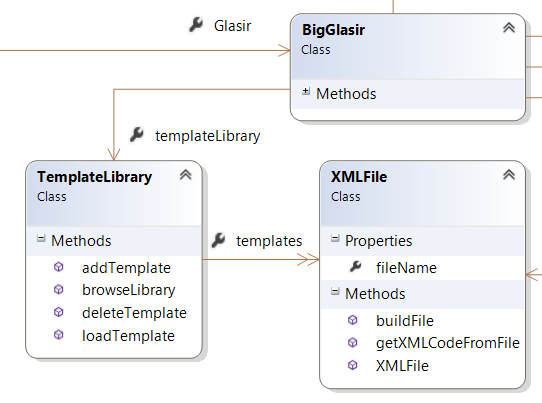
\includegraphics[width=0.8\textwidth]{figure/library.png}
            \caption{Diagramme de classes prévu pour la bibliothèque de modèles.}
            \label{fig:library}
        \end{figure}